\section{Architectural requirements}






\subsection{Quality Attributes workshop}
In this section we will present 8 phases of the QAW as described in \cite{BarbacciQualityAttribute2003}. Despite that a workshop is not held we still see clear benefits by using this model namely to determine the qualities for the electronic voting application before it is implemented. We are well aware that the outcome of the workshop is not perfect and will only cover the perspectives from a software developer and the security requirements. 

\begin{description}
    \item [QAW Presentation and Introductions]
        QAW facilitators describe the motivation for the QAW and explain each step of the method. 
    
    \item [Business/Mission Presentation]    
        A representative of the stakeholder community presents the business and/or programmatic drivers for the system.
    
    \item [Architectural Plan Presentation]
        A technical stakeholder presents the system architectural plans as they stand with respect to early documents, such as high-level system descriptions, context drawings, or other artifacts that describe some of the system's technical details.
    
    \item [Identification of Architectural Drivers]
     Architectural drivers often include high-level requirements, business/mission concerns, goals and objectives, and various quality attributes. During this step, the facilitators and stakeholders reach a consensus about which drivers are key to the system.
          
    
    \item [Scenario Brainstorm]
        Stakeholders generate real-world scenarios for the system. Scenarios comprise a related stimulus, an environmental condition, and a response. Facilitators ensure that at least one scenario addresses each of the architectural drivers identified in Step 4.
         
    \item [Consolidation] 
        Scenarios that are similar in content are consolidated.
    
    \item [Prioritization] 
  Stakeholders prioritize the scenarios through a voting process. 
    
    \item [Refinement]
        The top four or five scenarios are further clarified and the following are described:
        \begin{enumerate}
            \item the business/programmatic goals that are affected by those scenarios
            \item the relevant quality attributes associated with those scenarios   
        \end{enumerate}
\end{description}

\noindent
The above concludes the overview of the phases in the workshop. We will now use the structure of the phases to derive and define the QAS which will be the basic for our architecture. 

\subsubsection{3. Architectural Plan Presentation}
We will use this step to wrap up our first iteration for a high level overview of the system. This first overview is all based on the knowledge we got from the first part. We illustrate this overview through a component connector view. This viewpoint is concerned with the run-time functionality of the system.  At this point we have a component for a voter, tallier, observer, bulletin board and a registration process. We see the voter, tallier and the observers as clients and as active processes which all are communicating with the bulletin board. Therefor their must be a connector between the clients and bulletin board. The purpose of the registration authority is that every active participant must be registered through some registration authority before they can attend the electronic voting election. 

\begin{figure}[H]
\centering
     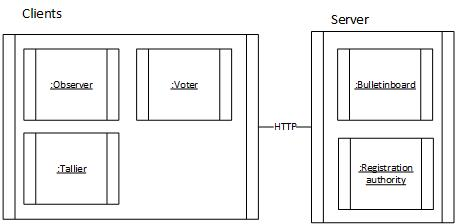
\includegraphics[scale=0.90]{CC_View_2.jpg}
     \caption{Initial draft of component \& connector viewpoint}     
\end{figure}
 


\subsubsection{4. Identify architectural drivers}
The purpose of this step is to identify architectural drivers. Architectural drivers are the keys to realizing quality attribute goals for the system. The architectural drivers are often found through requirements and business goals. We found architectural drivers by reflection and discussion against the security requirements of earlier described electronic voting application. Based on our architectural drivers, we begin to see the following quality attributes.\\


\begin{table}[H]
\centering
\begin{tabular}{|l|l|}
\hline
\multicolumn{2}{|l|}{Voters point of view}                \\ \hline
Usability    & \begin{tabular}[c]{@{}l@{}}The system should be easy to use for a voter \\ and give feedback \end{tabular}                  \\ \hline
Availability & \begin{tabular}[c]{@{}l@{}}The system should be available when needed \\ and if errors occours then the user should be \\ least affected by this. \end{tabular}                       \\ \hline
Interoperability         & \begin{tabular}[c]{@{}l@{}} A voter should be able to cast a vote \\ from a given device with a internet \\ connection\end{tabular}                                                                   \\ \hline

\end{tabular}
\caption{Voters point of view}
\end{table}


\begin{table}[H]
\centering
\begin{tabular}{|l|l|}
\hline
\multicolumn{2}{|l|}{Robustness}                                                                                                                                                                        \\ \hline
Performence         & \begin{tabular}[c]{@{}l@{}}Should be able to handle a large amount \\ of user within a reasonable time\end{tabular}                                                                   \\ \hline
Testability      & \begin{tabular}[c]{@{}l@{}}Given the nature of systems complexity it\\ should be easily testable to ensure \\ robustness and reliability\end{tabular}                                 \\ \hline
Security         & \begin{tabular}[c]{@{}l@{}}The integrity should withhold even though \\ if cheating occurs.\end{tabular}                                                                             \\ \hline
\multicolumn{2}{|l|}{Universal verifiability}                                                                                                                                                           \\ \hline
Interoperability & \begin{tabular}[c]{@{}l@{}}Not only participant but also passive observers \\ should be able to validate through out the \\ election and afterwards.\end{tabular}           \\ \hline

\multicolumn{2}{|l|}{Future proof}                                                                                                                                                                      \\ \hline
Modifiable       & \begin{tabular}[c]{@{}l@{}}Only a registered user should be able to vote. \\ This registration should be easily replaceable \\ depending on the nature of the election.\end{tabular} \\ \hline
Modifiable       & \begin{tabular}[c]{@{}l@{}}The system should modifiable such that\\  core elements are replaceable\end{tabular}                                                                      \\ \hline
\end{tabular}
\caption{Owners point of view}
\end{table}


\subsubsection{5. Scenario brainstorming}
The purpose of this step is to design QAS, based on our architectural drivers. That is, here we form QAS in a form such as described in \cite{Bass}. Here there should be a clear stimulus and response measurement.

\begin{longtable}[c]{|p{1.8cm}|p{8cm}|l|} 
\hline
Scenario \#      & Description   \\ \hline
1     & A user should be able to cast a vote under runtime and the PVSS client registers the vote with a confirm message, within 2 minutes experimentation. \\ \hline
2     & An internal crash occurs and the bulletin board is out of reach during normal operation. The response is that the error is logged and the system is running in degraded mode. The system should be up running within 5 minutes. \\ \hline
3     & A PVSS client cast a vote to the  bulletin board from a given device  with internet connection  under runtime and the system is updated and 100\% of the information is exchanged and processed correctly. \\ \hline
4     & An observer client validates a vote from the the bulletin board  under runtime. The validation is processed, and the bulletin board is updated and 100\% of the information is exchanged and processed correctly. \\ \hline
5      & 5 mill. users intiate their votes to the bulletin board under normal operation. The votes are processed and saved with average latency of 2 seconds. \\ \hline
6      & An unitester should be able to code a unit on the system under development and the test suite are executed  and result are captured and 85\% of the system are coverage  within 3 hours. \\ \hline
7       & A developer should be able to make a change to the registration code under  runtime and the change are made and tested within 3 hours.\\ \hline
8       & A developer should be able to make a change to the random number generator code under runtime and the change are made and tested within 3 hours.\\ \hline
9         & A cheater cast a invalid vote to the bulletin board under normal operation. All valid data should be preserved and the system should be able to detect invalid from  valid data before the total counting of the votes.\\ \hline

\caption{First step towards quality attributes scenarios}
\label{tab:myfirstlongtable}
\end{longtable}

\subsubsection{6. Scenario consideration}
The purpose of this step is to merge scenarios that have similar features. At the workshop there were no scenarios that could be merged.\\

\noindent
Usability is very vague described. It turns out that usability is closely related to modifiability in terms of preparing the architecture so the user interface can easily be replaced. Therefore, it's about building an architecture where business logic does not have a high coupling with the user interface, so one can easily add a new user interface. \\ 

\noindent
Scenario $3$ and $4$ are both about \textit{Interoperability}. We choose to merge scenario $4$ with scenario $3$, which means that scenario $4$ is removed. This means that scenario $3$ should contain the parts where the votes get validated. And of cause the scenario should take into account that an observer client should be able to communicate with the bulletin board.



\subsubsection{7. Scenario prioritization}
The purpose of this step is to draw up a priority list based on the total votes. The list is long but we will limit this thesis to focusing on a few and the rest we will comment. The list is primarily prioritized based on the security requirements.

\begin{description}
    \item [Scenario 3]
       There is focus on the fact that as many people as possible can access electronic voting application. One way to achieve this is to create the application as a web application. This ensure that everyone the have an internet connection and a device with a modern browser should be able to access the application. In addition to a web application, we want to ensure that as many devices as possible can communicate with our electronic voting system. One way to ensure this, is to construct a standardized interfacing which is compatible with different clients.
    
     \item [Scenario 9]
         Since the PVSS is a public verifiable protocol, there will be a high focus on fulfilling the \textit{Universal verifiability} requirement. This means if there are invalid votes they should be detected through public verification. The PVSS protocol has proves which ensures that if there is a "cheater" who cheats with their vote they will high with probability be discovered.
    
    \item [Scenario 6]
        To ensure \textit{Accuracy} as in that final tally is computed correctly, there will be high focus on ensuring the complex part of the code is testable. 
    
    \item [Scenario 7]    
        To ensure \textit{Eligibility} and \textit{Uniqueness} there will be high focus on creating a flexible registration module which first of all ensures authentication and authorization such that only registered voters can vote and only have permissions to vote one time. But the module should be flexible enough to be change to integrate to other registration data. 
        
     \item [Scenario 8]    
        There will be high focus on ensuring the \textit{Fairness} property regarding that none should be able to gain any knowledge of the outcome of the election. Also the \textit{Uncoercibility} property part regarding no one should be able to extract the value of a vote. Therefor the need to have a module which can generate/compute large numbers. The security can change over time and the need of computing larger numbers will therefor be a demand. The code should therefor be flexible if there is need for replacing the module with another number generator.       
     
    \item [Scenario 2]
        If the electronic voting application should be used by many participants then the architecture must be able to carry out the task it is supposed to do when needed. The architecture must be ready to mask or repair its errors within a given time period.
     
     \item [Scenario 5]
        If the electronic voting application should be used by many participants then the architecture must be ready to handle such a load. 
        
    \item [Scenario 1]
        The electronic voting application should be easy to use. One way of finding the best candidate to an user interface is to create usability test. Based on the test result we must be able to change the user interface with breaking the whole codebase. 
  \end{description}


\subsubsection{8. Scenario Refinement}
The purpose of this step is to form QAS, where divide into source, stimulus, artifact, environment, response and response measure. We will work on the first five of the scenarios. The rest can be found in appendex \ref{sec:the_remaining_qas:Availibility}, \ref{sec:the_remaining_qas:Performence} and \ref{sec:the_remaining_qas:Modifiability}.


\begin{table}[H]
\begin{center}
\begin{tabular}{|p{0.3cm}|p{2.5cm}|p{8cm}|}
  \hline
  \multicolumn{2}{|p{3cm}|}{\bfseries Scenario(s):} & \#  1: A PVSS client cast a vote to the bulletin board from a given device with internet connection  under runtime and the system is updated and 100\% of the information is exchanged  and processed correctly\\
  \hline
  \multicolumn{2}{|p{3cm}|}{\bfseries Relevant Quality Attributes:} & Interoperability\\
  \hline
  \multirow{6}{*}{\begin{sideways}{\bfseries Scenario Parts}\end{sideways}}
  & {\bfseries Source:} & A webbrowser \\
  \cline{2-3}
  & {\bfseries Stimulus:} & Cast a vote \\
  \cline{2-3}
  & {\bfseries Artifact} &  Bulletin board system \\
  \cline{2-3}
  & {\bfseries Environment:} &  Runtime \\
  \cline{2-3}
  & {\bfseries Response:} &  If the vote is valid it is accepted. If the vote is invalid it is rejected and the vote is removed from the bulletin board \\
  \cline{2-3}
  & {\bfseries Response Measure:} & 100 \% of the information is exchange and processed correctly \\
  \hline
\end{tabular}
\caption{Interoperability QAS}
\end{center}
\end{table}


\begin{table}[H]
\begin{center}
\begin{tabular}{|p{0.3cm}|p{2.5cm}|p{8cm}|}
  \hline
  \multicolumn{2}{|p{3cm}|}{\bfseries Scenario(s):} & \#  2: A cheater cast a invalid vote to the bulletin board under normal operation. All valid data should be preserved and the system should be able to detect invalid from  valid data before the total counting of the votes\\
  \hline
  \multicolumn{2}{|p{3cm}|}{\bfseries Relevant Quality Attributes:} & Security\\
  \hline
  \multirow{6}{*}{\begin{sideways}{\bfseries Scenario Parts}\end{sideways}}
  & {\bfseries Source:} & A cheater \\
  \cline{2-3}
  & {\bfseries Stimulus:} & Cast a invalid vote, with purpose of influencing the finale votes \\
  \cline{2-3}
  & {\bfseries Artifact} &  Bulletin board system \\
  \cline{2-3}
  & {\bfseries Environment:} &  Runtime \\
  \cline{2-3}
  & {\bfseries Response:} &  If the vote is valid it is accepted. If the vote is invalid it is rejected and the vote is removed from the bulletin board \\
  \cline{2-3}
  & {\bfseries Response Measure:} & 100 \% of the information is exchange and processed correctly \\
  \hline
\end{tabular}
\caption{Security QAS}
\end{center}
\end{table}


\begin{table}[H]
\begin{center}
\begin{tabular}{|p{0.3cm}|p{2.5cm}|p{8cm}|}
  \hline
  \multicolumn{2}{|p{3cm}|}{\bfseries Scenario(s):} & \#  3: An unitester should be able to code a unit on the system under development and the test suite are executed and result are captured and 85 \% of the system are coverage within 3 hours. \\
  \hline
  \multicolumn{2}{|p{3cm}|}{\bfseries Relevant Quality Attributes:} & Testability\\
  \hline
  \multirow{6}{*}{\begin{sideways}{\bfseries Scenario Parts}\end{sideways}}
  & {\bfseries Source:} & Unittester \\
  \cline{2-3}
  & {\bfseries Stimulus:} & Code unit completed \\
  \cline{2-3}
  & {\bfseries Artifact} &  Code \\
  \cline{2-3}
  & {\bfseries Environment:} &  Design time \\
  \cline{2-3}
  & {\bfseries Response:} &  Result captured\\
  \cline{2-3}
  & {\bfseries Response Measure:} & 85 \% path coverage in three hours\\
  \hline
\end{tabular}
\caption{Testability QAS}
\end{center}
\end{table}




\begin{table}[H]
\begin{center}
\begin{tabular}{|p{0.3cm}|p{2.5cm}|p{8cm}|}
  \hline
  \multicolumn{2}{|p{3cm}|}{\bfseries Scenario(s):} & \#  4:A developer should be able to make a change to the registration code under runtime and the change are made and tested within 3 hours \\
  \hline
  \multicolumn{2}{|p{3cm}|}{\bfseries Relevant Quality Attributes:} & Modifiability\\
  \hline
  \multirow{6}{*}{\begin{sideways}{\bfseries Scenario Parts}\end{sideways}}
  & {\bfseries Source:} & Developer \\
  \cline{2-3}
  & {\bfseries Stimulus:} & Needs to replace the registration module \\
  \cline{2-3}
  & {\bfseries Artifact} &  Code \\
  \cline{2-3}
  & {\bfseries Environment:} &  Design time \\
  \cline{2-3}
  & {\bfseries Response:} &  Replacement made and Unit tested\\
  \cline{2-3}
  & {\bfseries Response Measure:} & In three hours\\
  \hline
\end{tabular}
\caption{Modifiability QAS}
\end{center}
\end{table}



\begin{table}[H]
\begin{center}
\begin{tabular}{|p{0.3cm}|p{2.5cm}|p{8cm}|}
  \hline
  \multicolumn{2}{|p{3cm}|}{\bfseries Scenario(s):} & \#  5: A developer should be able to make a change to the random number generator code under runtime and the change are made and tested within 3 hours. \\
  \hline
  \multicolumn{2}{|p{3cm}|}{\bfseries Relevant Quality Attributes:} & Modifiability\\
  \hline
  \multirow{6}{*}{\begin{sideways}{\bfseries Scenario Parts}\end{sideways}}
  & {\bfseries Source:} & Developer \\
  \cline{2-3}
  & {\bfseries Stimulus:} & Needs to replace the random generator \\
  \cline{2-3}
  & {\bfseries Artifact} &  Code \\
  \cline{2-3}
  & {\bfseries Environment:} &  Design time \\
  \cline{2-3}
  & {\bfseries Response:} &  Replacement made and Unit tested\\
  \cline{2-3}
  & {\bfseries Response Measure:} & In three hours\\
  \hline
\end{tabular}
\caption{Modifiability QAS}
\end{center}
\end{table}








\subsection{Tactics}
This section is about tactics which satisfies the QAS derived from the QAW. A tactic is a design decision that influences the achievement of a quality attribute response. We will discuss our choosen tactics based on our QAS developed from the QAW. We will describe them in the same order in which they are arranged above. For each tactic there will be a description and an argument of the choosen tactic. Depending on the tactics, we will complement with the necessary views that affect the architecture including module-, component and connector- or allocation viewpoint. 


\noindent
\subsubsection{Interoperability} \label{sec:interoperability:restapi}
This QA is related to QAS 1. Interoperability is about how systems meaningfully exchange information through interfaces in a given context. Since there will be different devices interacting with the bulletin board there is a demand on designing a standard interface which can serve these devices. \textit{Discover Service} stands for the location of a data exchange service and that it is visible to those who need it. The service can be located by type of service, by name, by location or by some other attribute.

\begin{figure}[H]
\centering
    \makebox[\textwidth]{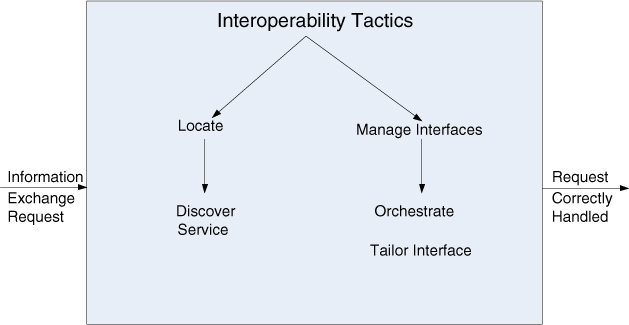
\includegraphics[scale=0.60]{tactic_interoperability.jpg}}
  \caption{Interoperability tactics \cite{Bass}}   
\end{figure}


\noindent
With \textit{Discover service} we will create a clear line between clients and the bulletin board. We will implement a REST API for this tactic.\\

\noindent
\textbf{REST - Representation State Transfer}\\
The idea behind REST is that every resource has it’s own URL (name) and you use the different HTTP methods to interact with those resources. REST consists of set of principles \cite{Fielding}, but we will only use a subset of these principles as follows.

\begin{enumerate}
    \item Transferring a representation of data in a format matching one of standard data types such as JSON, XML, HTML etc.
    \item A resource is information that is identified by a URL provided by the server. A URL is Uniform Resource Locator which describe the address of a particular resource on the internet.
    \item Interactions are stateless where each request contains all the information necessary. This is because of the scaling property.
\end{enumerate}


\noindent
The HTTP methods such as GET, POST, PUT and DELETE allow us to interact with the resources through an interface.



\noindent
\subsubsection{Security}
This QA is related to QAS 2. Security is concerned with the ability to protect data and information from unauthorized access while still providing access to people/systems that are authorized. The PVSS protocol ensures that only valid votes are accepted and counted. This prevents that invalid votes are counted in the final counts and thereby they will not effect the result. The \textit{Verify message integrity} tactic employs techniques such as checksums or hash values to verfy the integrity of a message. After the system has detected an attack the system must react on the attack.


\begin{figure}[H]
\centering
    \makebox[\textwidth]{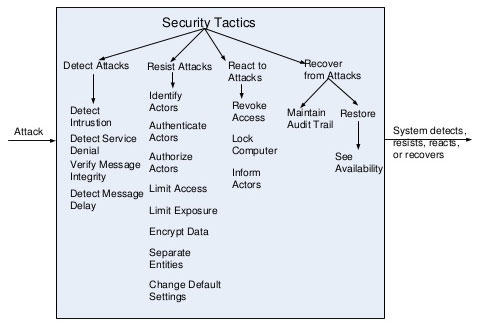
\includegraphics[scale=0.80]{tactic_security.jpg}}
  \caption{Security tactics \cite{Bass}}   
\end{figure}

\noindent
The $DLEQ$ and $PROOF_U$ proofs verifies the message integrity. With the proofs the protocol will be able to detect attacks. The verify message integrity consists of:

\begin{enumerate}
    \item The $DLEQ$ proof provided in ballot casting process ensures consistency in the encryption process.
    \item  The $PROOF_U$ ensures that the voter votes either 0 or 1.
    \item  The $DLEQ$ proof in the tallying process ensures that the decryption is done correct.
\end{enumerate}

\noindent
As already described this tactic is a part of the protocol which is described in section \ref{sec:proofs}. We use the \textit{Verify message integrity} tactic in relation with the proofs which ensures that the vote is either 0 or 1 and that the shares are constructed correctly and consistent. Our work consists of realizing the tactic in code. Another important decision to make, is if an attack is detected then the system, must react. The tactic \textit{Inform actors} includes other systems to be notified. One way could be marking the vote in the database as not valid. The means that the vote is not counted in the tallying phase.\\   

\noindent
\textbf{Component and Connector viewpoint}\\
This viewpoint shows the runtime functionality regards how responsibility are flows in creating and verifying the proofs between the prover, bulletin board and the verifier. 

\begin{figure}[H]
\centering
     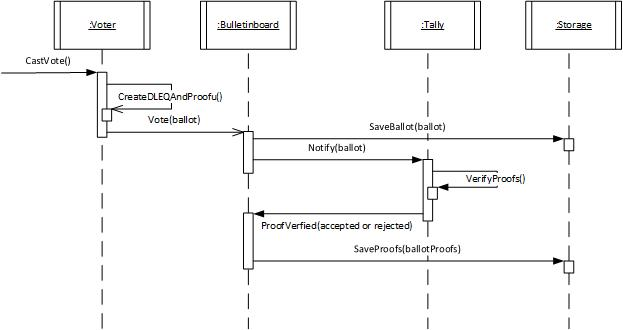
\includegraphics[scale=0.65]{security_proofs.jpg}
     \caption{Sequence diagram which shows an overall flow of verifying the proofs}     
\end{figure}


\begin{description}
    \item[Step 1] The vote is casted and the voter creates the data for the proofs. The voter is an active process which the double bars on the box indicates. The voter is active process because it constantly awaits input from the user.  

    \item[Step 2] The bulletin board recieves the ballot from the voter. It saves the ballot into a storage. It notifies the tally with the ballot. The bulletin board is an active process since it always listen on a specific port with purpose to serve incoming request.   
    
    \item[Step 3] The tally verifies the proofs and revoke a method on the bulletin board with a parameter which indicate if the proof was accepted or rejected. For now we have choosen that the tally is an active process under the entire election. 
    
    \item[Step 4] The bulletin board saves the ballot proof into a storage. We will emphasize that we always saves and never update. This constraint helps the system resist unauthorized users from updating any data in the storage. The storage is an active process because it constantly awaits incoming request.  

\end{description}


\subsubsection{Testability}
This QA is related to QAS 3. Testability is concerned with the ease with which the software can be made to demonstrate its faults. This application contains a fair amount of computation which is the core of the application - namely to compute the final votes. Testing is needed, to ensure accuracy of the computations. When new features are introduced to the system, one should be able to execute all tests and results are captured and 85 \% of the system are coverage within 3 hours.


\begin{figure}[H]
\centering
      \makebox[\textwidth]{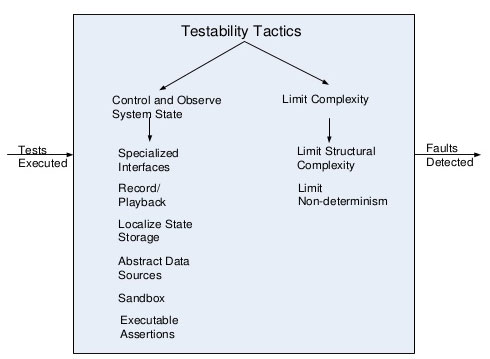
\includegraphics[scale=0.60]{tactic_testability.jpg}}
  \caption{Testability tactics \cite{Bass}}   
\end{figure}



\noindent
The Voter client is build in Javascript which means that we have to adapt to the opportunities (dynamic, untyped, and interpreted run-time language) which the language provides. This tactic will be limited to webclient since they contain all computations. The tactic \textit{Limit structural complexity} is about isolating, encapsulating dependencies and reduce dependencies between components. These principles leads to limited complexity and thereby better testability.   \\

\noindent
 For a system to be testable we need to be able to control components inputs and be able to change its internal state and then observe its output. One of the ways for achieving this is through various design patterns such a strategy pattern. In general one should strive to use composite patterns that encapsulates responsibility which we use in section \ref{sec:modifiability_random_generator}  \\


\noindent
\textbf{Component and Connector viewpoint}\\
Figure ~\ref{fig:voterclient_functions_which_needs_to_be_testable}  shows the flow on the Voter client of the various functions which need to be executed in order to compute the ballot casting and proofs.

\begin{figure}[H]
\centering
      \makebox[\textwidth]{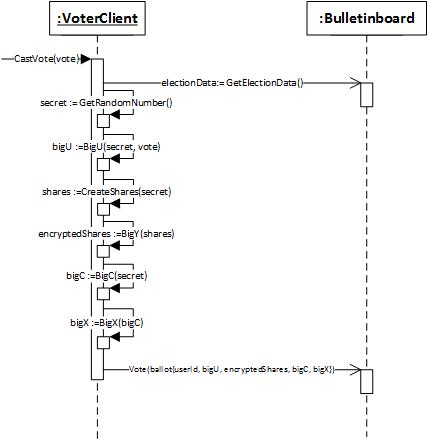
\includegraphics[scale=0.70]{testing_sequencediagram.jpg}}
  \caption{Voter client functions which needs to be testable}  
   \label{fig:voterclient_functions_which_needs_to_be_testable}
\end{figure}


\noindent
All functions ought to be relatively easy to test because they are fairly isolated. The communication with the bulletin board can be abstracted away in a testing environment through Test stubs \cite{Baerbak10}. 


\subsubsection{Modifiability} \label{sec:modifiability_registations_process}
This QA is related to QAS 4. Modifiability is concerned with the ease with which the system supports change. In a reel electronic voting application scenario there will be need of a certain registration process. Depending on the scenario the registration process may go through state authorities, google, linkedin or even a third solution. Therefor the system must be able to support changes on the registration process depending on the use. 

\begin{figure}[H]
\centering
    \makebox[\textwidth]{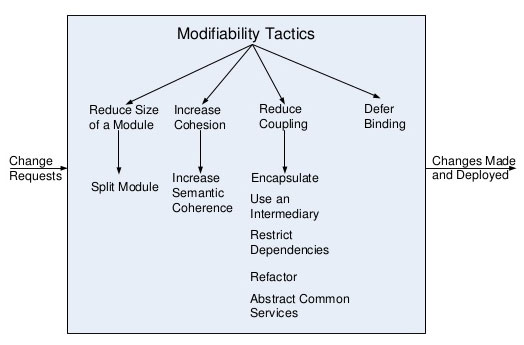
\includegraphics[scale=0.60]{tactic_modifiability.jpg}}
  \caption{Modifiability tactics \cite{Bass}}   
  \label{fig:modifiability_tactic}
\end{figure}


\noindent
\textbf{Module viewpoint}\\
Figure ~\ref{fig:the_registrations_process} shows the module viewpoint of a the strategy pattern on the process of registering a voter.


\begin{figure}[H]
\centering
    \makebox[\textwidth]{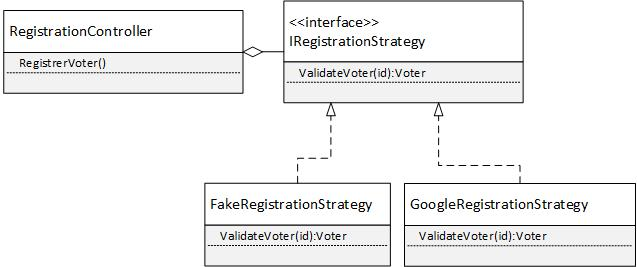
\includegraphics[scale=0.60]{registration_classdiagram.jpg}}
  \caption{Module viewpoint of the strategy pattern on the registrations process} 
   \label{fig:the_registrations_process}
\end{figure}
\noindent
The RegistgrationsController gets an instance of the type IRegistrationStrategy. It can either be an instance of a GoogleRegistrationStrategy or a FakeRegistgrationStrategy. Each of these classes has their implementation of the method ValidateVoter. The GoogleRegistrationStrategy should implement a registration process to Google API. The FakeRegistgrationStrategy just contain "true" which means that the voter is a valid voter in the registration process. This strategy is only meant for testing purposes. \\ 

\noindent
The process which led to this pattern is the compositional process which is as follows.

\begin{description}
    \item[Identify the behavior that varies:] In this case it is the registration process.  

    \item[Use interface which encapsulate the variable behavior:]  In this case we create an interface IRegistrationStrategy which defines a  responsibility of registering a voter.     
    
    \item[Delegate the responsibility to a specialized classes:] In this case we have FakeRegistgrationStrategy and a GoogleRegistrationStrategy.
\end{description}

\noindent
By implementing a strategy pattern on the registration process, we have used the tactic \textit{Encapsulate} and efficiently encapsulated this functionality and made the system ready to change to other registration authorities. Answering the question if we are able to reach the response measure from the QAS, depends on how complicated it is to integrate against an external registration system. 


\subsubsection{Modifiability} \label{sec:modifiability_random_generator}
This QA is related to QAS 5.  As described modifiability is concerned with the ease with which the system supports change. To further prove the security of the implementation we must take into account that the random generator easily can be changed. This is an advantage if we need to work with, for example, larger numbers in the future. \\ 


\noindent
The tactic \textit{encapsulate}, from figure \ref{fig:modifiability_tactic}, reduces the coupling between modules. The goal is to create an interface to the number generate so that we are able to shield of the concrete implementation of a given number generator and thereby reduce the coupling between modules. If  we later then need to change the implementation we can create a new implementation of the number generator and  replace the old one. \\





\noindent
This tactic is limited to webclient since they contain all computations and the number generator. The following will be a proposal for an implementation of the concrete number generator and how one can encapsulate it with an interface.\\


\noindent
\textbf{Module viewpoint}\\
This viewpoint shows the use of a strategy pattern as described in \cite{Baerbak10}. The idea with the strategy pattern is to define a family of business rule, encapsulate each one and make them interchangeable. The strategy pattern lets the business rules vary independently from clients that use it. It delegates the responsibility to an object instead of doing the work it self. 



\begin{figure}[H]
\centering
    \makebox[\textwidth]{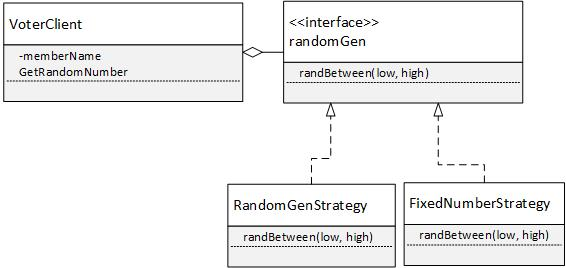
\includegraphics[scale=0.60]{M_View_RandomNumberGenerator.jpg}}
  \caption{Module viewpoint of the strategy pattern on the random number generator} 
  \label{fig:the_random_number_generator}
\end{figure}


\noindent
Figure ~\ref{fig:the_random_number_generator}  shows the VoterClient gets an instance of a randomGen which has a method randBetween. It can either be an instance of a RandomGenStrategy or a FixedNumberStrategy. Each of these classes has their implementation of the method randBetween. The RandomGenStrategy implements the reel random number generator. The FixedNumberStrategy returns a controlled value which we can set, for testing purposes.\\

\noindent
The process which leds to this pattern is the compositional process which is as follows.


\begin{description}
    \item[Identify the behavior that varies:] In this case it is the random number generator.  

    \item[Use interface which encapsulate the variable behavior:]  In this case we create an interface randomGen which defines a  responsibility of returning a random number.     
    
    \item[Delegate the responsibility to a specialized classes:] In this case we have RandomGenStrategy and a FixedNumberStrategy.
\end{description}

\noindent
By implementing a strategy pattern it should be relative easy to switch out the random number generator and thereby making changes to this part of the system.